\section{Evaluation}
\label{sec:evaluation}

In this section, we report experimental results of our homomorphic bloom filter protocols based on a real-world mobile data access dataset. First, we briefly describe the dataset and the experimental setup. Next, the parameter settings of the protocols used in our experiments are presented. Then, we compare the computation and communication overhead of different protocols. Finally, we explore the impacts of Geohash length on the computing efficiency as well as the security.

\subsection{Datasets and Experimental Setup}
Our dataset consists of multiple mobile data access traces of smartphone users in a small city in China. More specifically, this dataset includes 7607 unique users, 121 cell towers, and is collected from 6:00 pm to 9:00 pm on a Sunday in 2014. Each mobile data access record contains the coordinate of the cell tower with which the user communicates. A sequence of records of a user can be viewed as her history trajectory. We randomly pick users and generate queries for evaluation. All experiments are performed on a PC with a 3.10GHz Xeon E3-1220 processor, and 32GB memory,
running Red Hat 4.8.5.

\begin{figure*}[t]
	\centering
	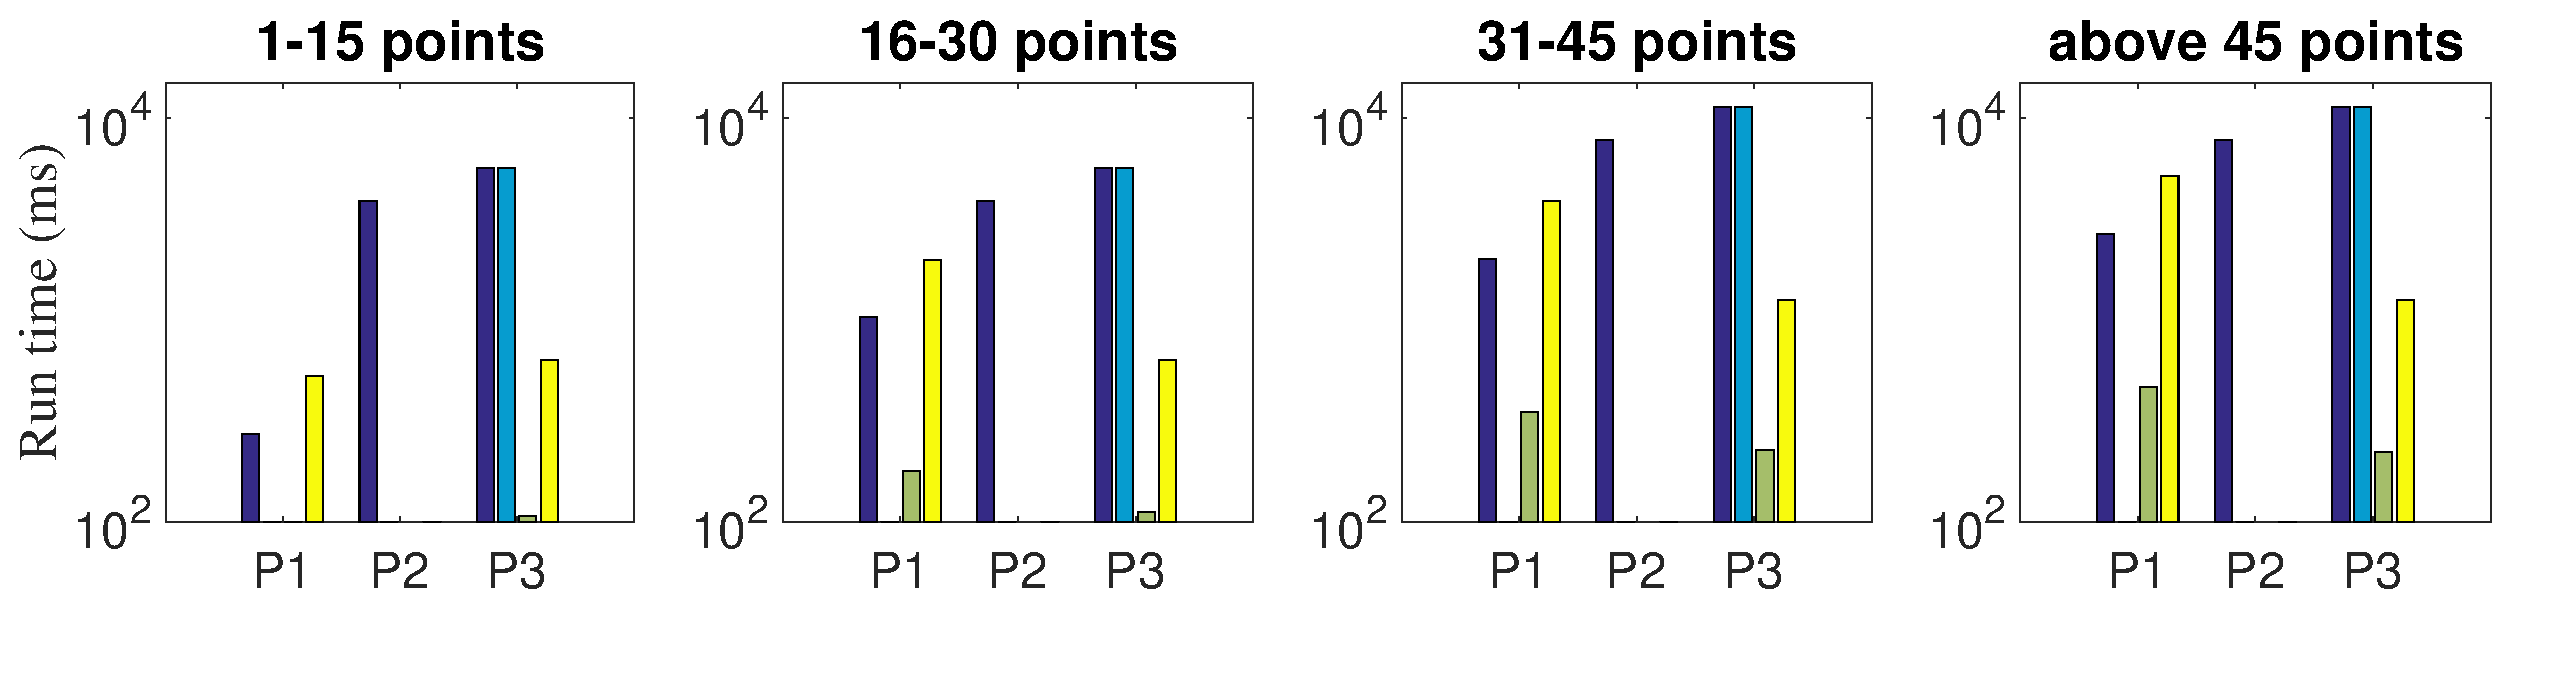
\includegraphics[width=\linewidth]{figures/computation_oh.pdf}
	\caption{Computation overhead.}
	\label{fig:computation_oh}
\end{figure*}

\subsection{parameter settings}
We group users in our dataset into 4 categories, by their number of unique visited location points: 1-15 points, 16-30 points, 31-45 points, above 45 points. According to number of unique location points of each group, we set the bloom filter parameters according to~\autoref{equ:k} and~autoref{equ:m}. The desired false positive probability is set as 0.1. We use 250 bit bloom filter with 4 hash function for group 1 \& 2, i.e., users with fewer visited location points than 30. We use 500 bit bloom filter with 4 hash function for group 3 \& 4, i.e., users with more visited location points than 30.

We implement our design both on an integer encryption system (SEAL) and a binary encryption system based on ~\cite{van2010fully}. More specifically, Protocol 1 and Protocol 2 are implemented on integer encryption system, while Protocol 3 is implemented on binary encryption system. As mentioned in \ref{sec:para_sele}, we set polynomial modulus as $``1x \,\hat{}\, 1024 + 1"$, coefficient modulus as $FFFFFFF00001$ and plaintext modulus as $256$. Under this setting, we calculate the size of a freshly encrypted integer in SEAL as $1025*48*2 = 98400$ bits, where $1025$ is the number of coefficients in one polynomial, $48$ is the number of bits per coefficient occupies, and $2$ is the size of the array of polynomials. To minimize difference of the size of cipertext, for binary encryption system, the security parameter $\lambda$ is set as 4, and each bit in the plaintext is encrypted into 1024-bit wide ciphertext.

\subsection{computation overhead}
The computation overhead can be decomposed to three part: the encryption time, the query computation time and decryption time, where encryption happens at both A and B. We randomly perform 20 queries for each group of users and compare the computation overhead of all three protocols in \autoref{fig:computation_oh}. 

As you can see that in protocol1 (P1) encryption overhead at A is much larger than encryption overhead at B as the number of integers to be encrypted relates to the number of elements inserted into the bloom filter. Such a relation is also the reason why the encryption overhead increase as the number of location points increase. Since protocol1 also incur large intermediate results to be transmit back to A, so the decryption overhead is also very high which can reach 5 seconds. In protocol2 (P2), the encryption overhead at A dominates the overall computation overhead which can reach 8 seconds. As the data at B and intermediate results are both very short. The computation overhead of protocol3 (P3) can reach 24 seconds in total (11 seconds for encryption) which is the highest among all three protocols, mainly because the encryption method is different (bitwise encryption). All three protocols show a same trend is that the computation overhead are mainly caused by encryption/decryption whereas the query computation has very limited contribution towards the overall computation overhead.

\subsection{communication overhead}
The communication overhead consist of three parts: send ciphertext from A and B to server, retrieve computation results from cloud to A, A send query result to B. Since the last part is transmitted in plaintext and the size is negligible, so we focus on the first two parts in our evaluation. 

We use the size of the ciphertext to be transmitted as the main measure for communication overhead. We compare the communication overhead of all three protocols in \autoref{fig:communication_oh}.

\begin{figure*}[h]
    \centering
    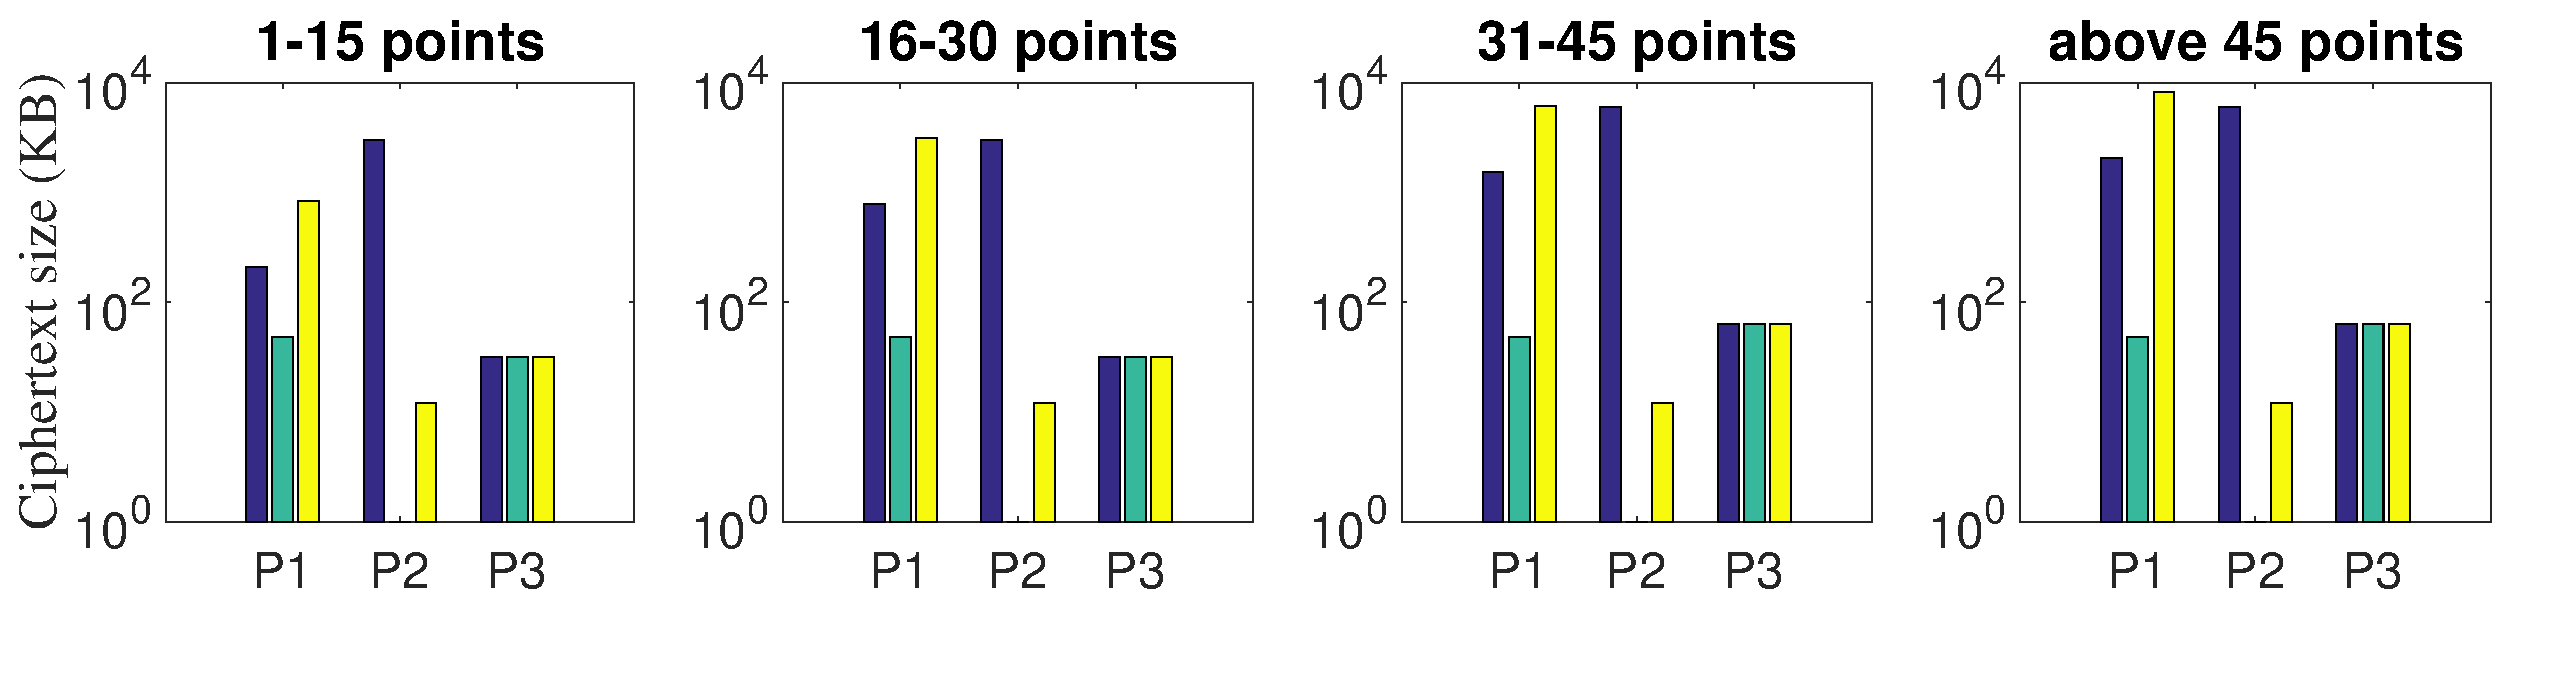
\includegraphics[width=\linewidth]{figures/communication_oh.pdf}
    \caption{Communication overhead.}
    \label{fig:communication_oh}
\end{figure*}

As you can see that in protocol1 (P1), beside large communication overhead at transmitting ciphertext form A to server, the communication overhead of transmit intermeidate results are also very high as large number of ciphertext is created by the query computation. The highest overhead reaches 2MB. For protocol2 (P2), most of the overhead happens at sending ciphertext from A to server, as each bit in the bloom filter is treated as an integer. The communication overhead of protocol2 is the highest among all three protocols which can reach 6MB. Protocol3 (P3) which adopts a bitwise encryption scheme, has the lowest communication overhead with only tens of KB in size. 

\subsection{the accuracy}
As the bloom filter has possible false positives. We evaluate here the with different required false positive possibility $p$, how are the overhead changes. We show the trend of the computation overhead in \autoref{fig:accuracy_comp} and the communication overhead in \autoref{fig:accuracy_comm}.

For protocol1 (P1), we can see that the both computation overhead and communication overhead mainly decreases as $p$ increases with the exception that the encryption overhead at B is stable as it require constant time. For protocol2 (P2), as the encryption at A and transmit data from A to server dominate the computation overhead and communication overhead respectively, they both decreases as $p$ increases, where as other overheads are quite stable. Similar to protocol1 and protocol2, protocol3 also shows a trend of decreasing overhead as $p$ increase.

\begin{figure*}[h]
    \centering
    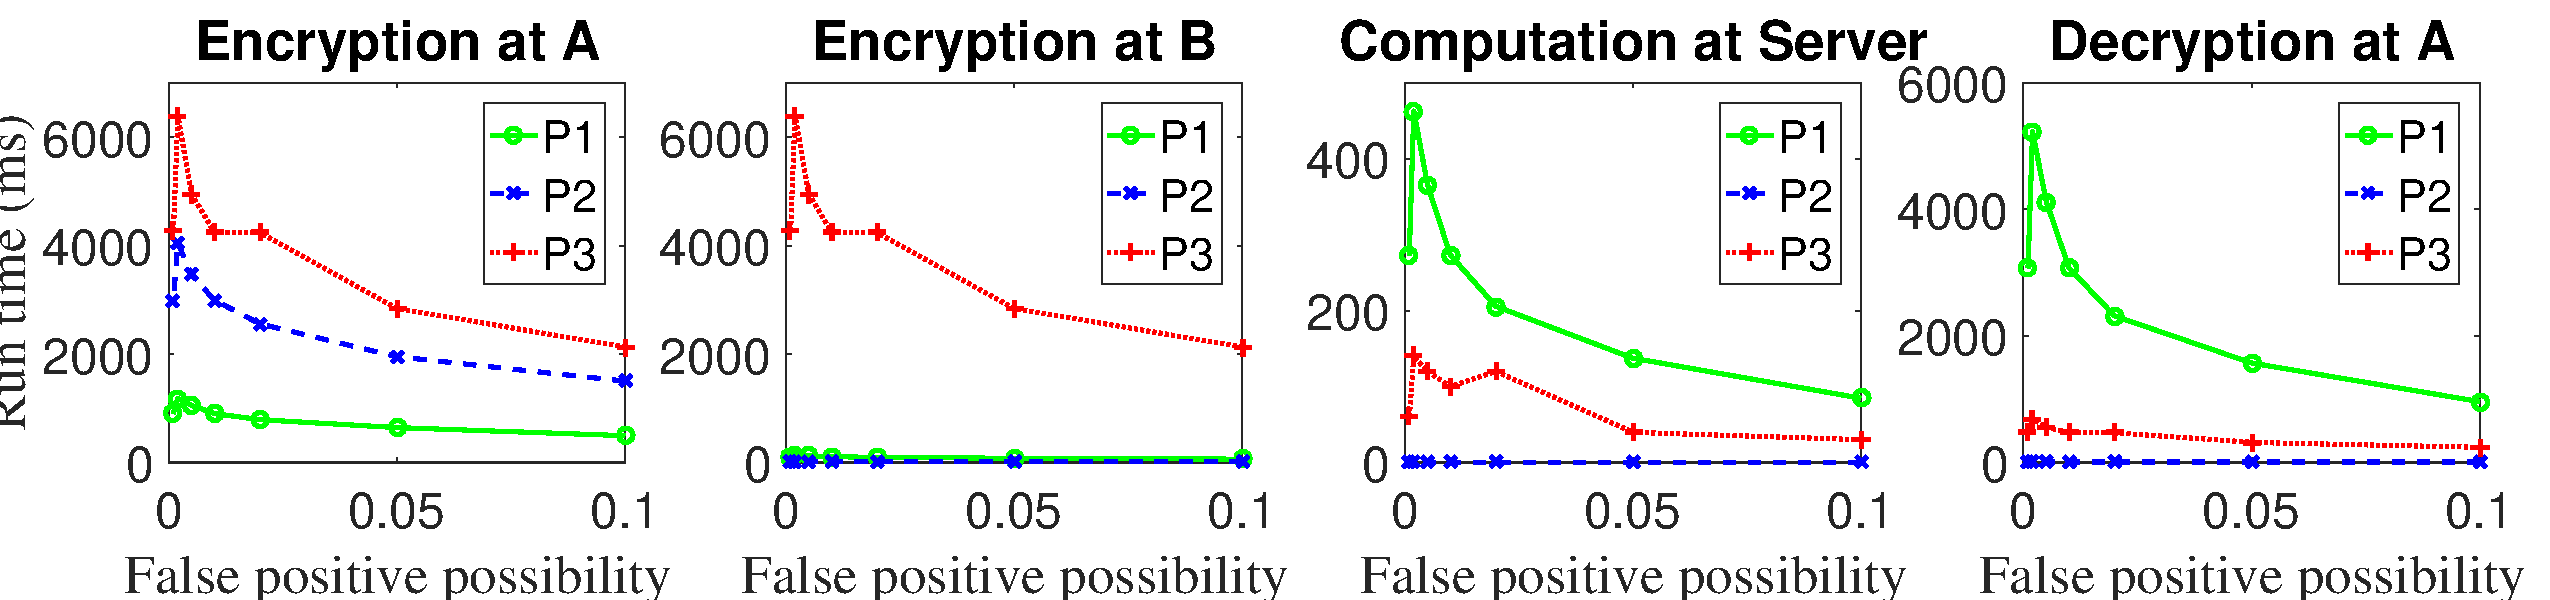
\includegraphics[width=\linewidth]{figures/accuracy_comp.pdf}
    \caption{Accuracy vs computation overhead.}
    \label{fig:accuracy_comp}
\end{figure*}


\begin{figure*}[h]
    \centering
    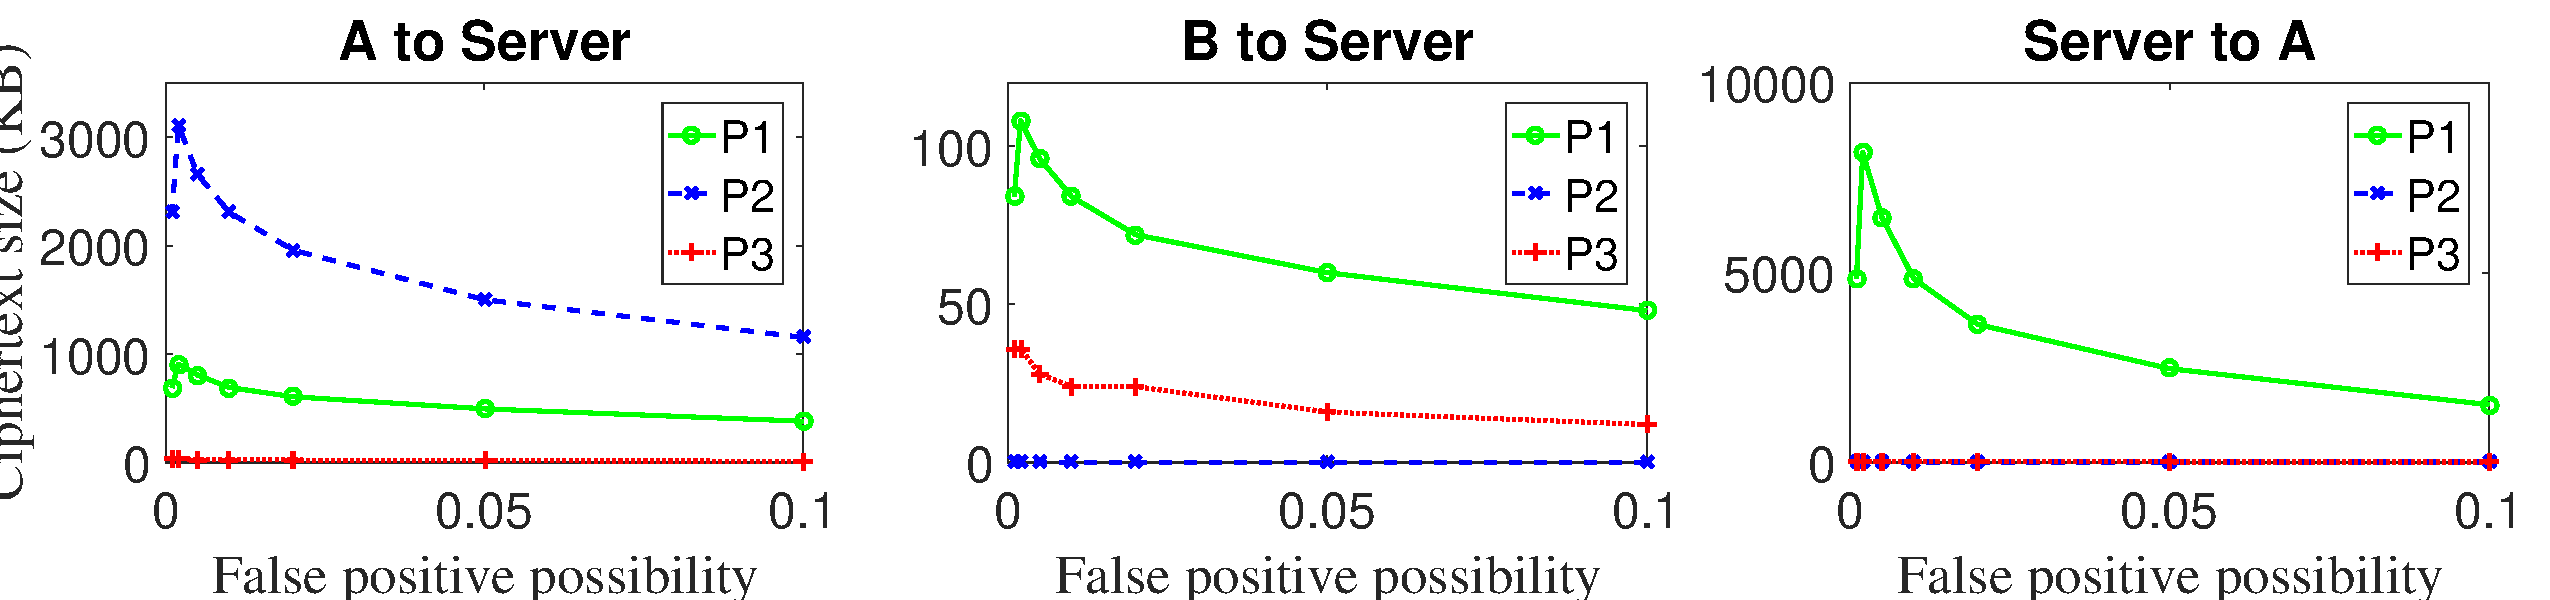
\includegraphics[width=\linewidth]{figures/accuracy_comm.pdf}
    \caption{Accuracy vs communication overhead.}
    \label{fig:accuracy_comm}
\end{figure*}

\subsection{geohash efficiency}
Geohash help to reduce both computation overhead and communication overhead compared to regular version. We evaluate the relation of the size of regions and reduction in overheads. Various region size are used and results are shown in \autoref{fig:geohash}.

By sending geohash values in plaintext, B also possibly reveal his location information to A. The possibility of reveal the exact location highly related to the number of location points in each region.

Figure \ref{fig:geohash_eval} illustrates the bloom filter size required to keep the false positive rate $p$ not larger than 0.01, and the probability of leaking private locations during the query with various Geohash lengths. We assume the locations are evenly distributed and there is exactly one location distributed in the area of 1m x 1m, 10m x 10m, 100m x 100m and 1km x 1km respectively. Take the 1m x 1m and the Geohash length of 6 as an example. Since exactly only one location in each 1m x 1m area, the Geohash with a length of 6 covers an area of 1.22km x 0.61km, which can be found in Table \ref{tab:geohash_region_size}, containing $n$= 1220x610 locations, i.e., elements. Therefore, the size of bloom filter can be calculated by Equation \ref{equ:m}, and the probability of leaking the location can be expressed by $1/n$;

\begin{figure}[h]
    \centering
    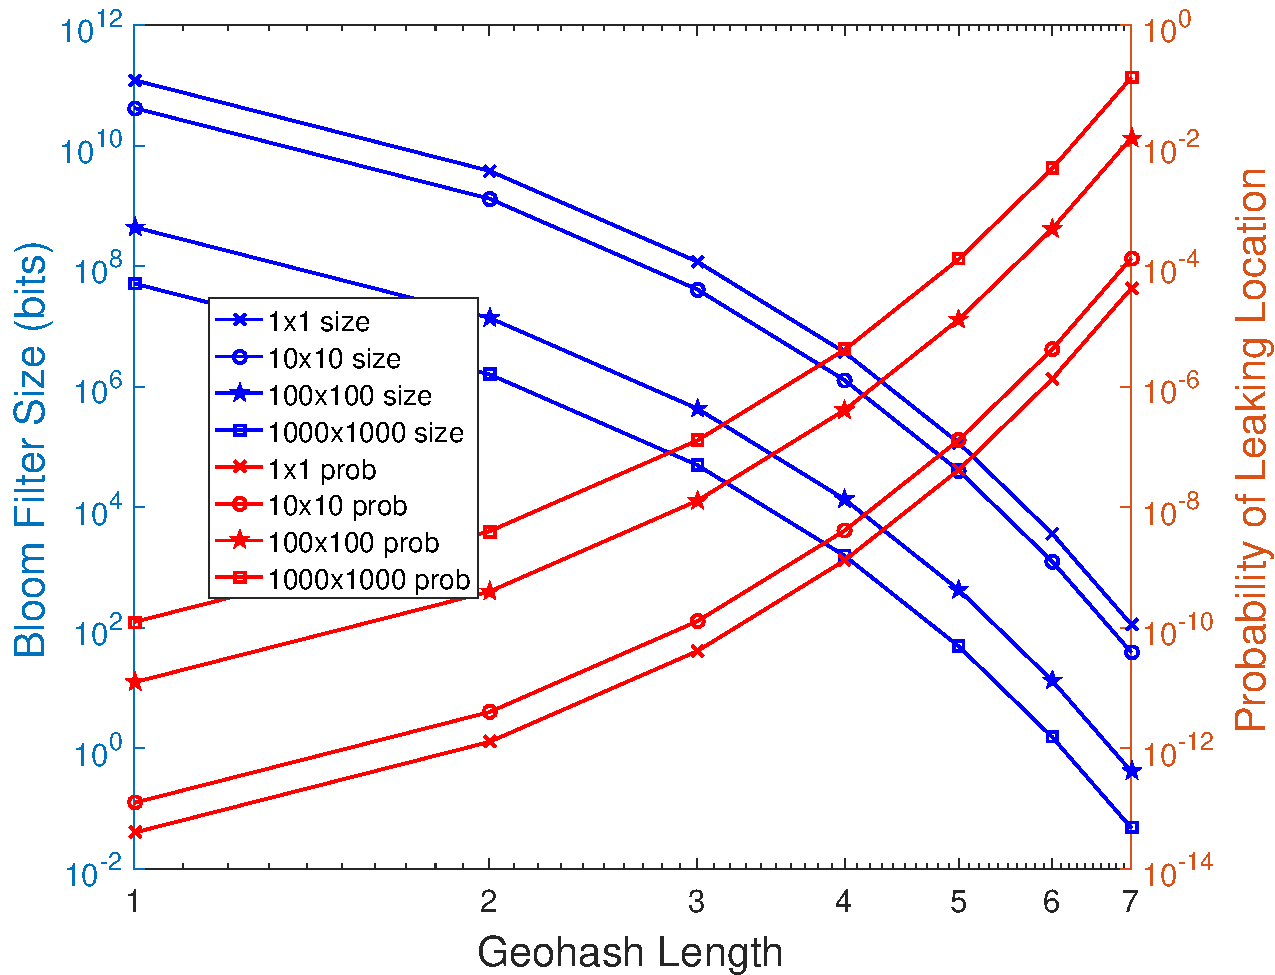
\includegraphics[width=0.7\linewidth]{figures/geohash_eval.pdf}
    \caption{Geohash.}
    \label{fig:geohash_eval}
\end{figure}

